\section*{Problema P9.69}

\renewcommand*\thesection{9.69}
\numberwithin{equation}{section}

\begin{center}
    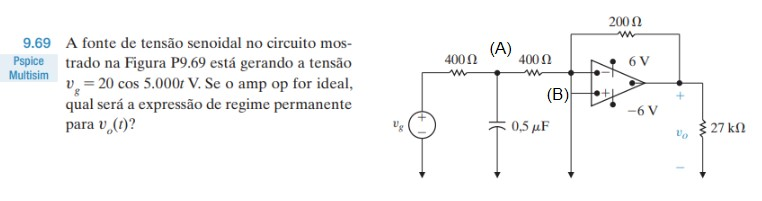
\includegraphics[scale=1.0]{P9.69.jpg}
\end{center}

O primeiro passo é expressar $V_o$ em função das tensões de entrada no AmpOp.
Aplicamos análise nodal no nó $(B)$.

\[ i_- + i_+ + i_{GND} + \frac{V_B - V_o}{R_s} + \frac{V_B - V_A}{R_2} = 0 \]

Como o Amplificador Operacional é ideal, temos

\begin{equation}\label{eq:9.69.1}
    i_- = i_+ = 0 \un{A}
\end{equation}

Além disso, temos $V_B = 0$. Substituindo na expressão do nó, temos

\[ i_{GND} + \frac{V_o}{R_s} + \frac{V_A}{R_2} = 0 \]

Isolando $V_o$, temos

\begin{equation}\label{eq:9.69.2}
    V_o = - R_s\left(i_{GND} + \frac{V_A}{R_2}\right)
\end{equation}

Agora aplcamos análise de malhas, com as correntes de malha $i_1$ e $i_2$ na figura. Note que $i_2 = i_{GND}$. \\
Começamos pela malha 1:

\[ -V_g + R_1i_1 + \frac{1}{j\omega C}(i_1 - i_2) = 0 \]

\[ R_1i_1 - \frac{j}{\omega C}(i_1 - i_2) = V_g \]

\[ i_1\left(R_1 - \frac{j}{\omega C}\right) + i_2\left(\frac{j}{\omega C}\right) = V_g \]

Agora vamos para a malha 2:

\[ \frac{1}{j\omega C}(i_2 - i_1) + R_2i_2 = 0 \]

\[ i_1\left(\frac{j}{\omega C}\right) + i_2\left(R_2 - \frac{j}{\omega C}\right) = 0 \]

Com as duas equações de malha, temos o sistema linear

\begingroup
\renewcommand*{\arraystretch}{3}

\begin{equation}\label{eq:9.69.3}
    \begin{bmatrix}
        R_1 - \frac{j}{\omega C} & \frac{j}{\omega C}     \\
        \frac{j}{\omega C}     & R_2 - \frac{j}{\omega C}
    \end{bmatrix}
    \begin{bmatrix}
        i_1 \\
        i_2
    \end{bmatrix}
    =
    \begin{bmatrix}
        V_g \\
        0
    \end{bmatrix}
\end{equation}
\endgroup


Substituindo os valores, temos

\begingroup
\renewcommand*{\arraystretch}{3}

\[
    \begin{bmatrix}
        400 - j400 & 400       \\
        400      & 400 - j400
    \end{bmatrix}
    \begin{bmatrix}
        i_1 \\
        i_2
    \end{bmatrix}
    =
    \begin{bmatrix}
        \frac{5000}{\sqrt{2}} \\
        0
    \end{bmatrix}
\]

\[
    \begin{bmatrix}
        400 - j400 (400 + j400) & 400    (400 + j400)    \\
        400      & 400 - j400
    \end{bmatrix}
    \begin{bmatrix}
        i_1 \\
        i_2
    \end{bmatrix}
    =
    \begin{bmatrix}
        \frac{5000}{\sqrt{2}} (400 + j400) \\
        0
    \end{bmatrix}
\]

\[
    \begin{bmatrix}
        320000 & 400    (400 + j400)    \\
        400      & 400 - j400
    \end{bmatrix}
    \begin{bmatrix}
        i_1 \\
        i_2
    \end{bmatrix}
    =
    \begin{bmatrix}
        \frac{5000}{\sqrt{2}} (400 + j400) \\
        0
    \end{bmatrix}
\]

\[
    \begin{bmatrix}
        320000 & - 400    (400 + j400)    \\
        0      & 400 - j400 + \frac{400(400 + j400)}{-800}
    \end{bmatrix}
    \begin{bmatrix}
        i_1 \\
        i_2
    \end{bmatrix}
    =
    \begin{bmatrix}
        \frac{5000}{\sqrt{2}} (400 + j400) \\
        0 + \frac{\frac{5000}{\sqrt{2}} (400 + j400)}{-800}
    \end{bmatrix}
\]

\endgroup

Resolvendo, temos

\[ i_2 = \frac{\frac{\frac{5000}{\sqrt{2}} (400 + j400)}{-800}}{400 - j400 + \frac{- 400(400 + j400)}{-800}} \]

\[ i_2 = \frac{\frac{5000}{\sqrt{2}} (400 + j400)}{-320000 + j320000 - 400(400 + j400)} \]

\[ i_2 = \frac{1414200 + j1414200}{-480000 + j160000} \]

\[ i_2 = \frac{2\cdot10^6\phase{45^{\circ}}}{505964\phase{161.57^{\circ}}} \]

\begin{equation}\label{eq:9.69.4}
    i_2 = i_{GND} = 3,95\phase{-116,57^{\circ}} \un{A}
\end{equation}


    























